\section{Модификация проекта <<Изображение проекции полиэдра>>}

\subsection{Постановка задачи}

Модифицируйте эталонный проект таким образом, чтобы определялась и печаталась следующая характеристика полиэдра: сумма площадей граней, все вершины которые расположены вне сферы.

После запуска программы, программа вычисляет площадь полигонов, которые расположены вне сферы.
Это задание не требует серьёзной модификации исходного кода, все функции будут вписываться в файл проекта \verb|polyedr.rb|.

\subsection{Решение}

Для выполнения задания необходимо определить хорошую точку в пространстве,если она строго находится вне сферы $x^2+y^2+z^2=1$.  Вычислить сумму площадей граней, все вершины которые расположены вне сферы $x^2+y^2+z^2=1$.



\subsection{Модификация кода}

Создадим метод модуля.

\begin{small}
\begin{verbatim}
 def length
    Math.sqrt(@x*@x + @y*@y + @z*@z)
 end
\end{verbatim}
\end{small}

Метод, который вычисляет вершины, который лежат вне сферы $x^2+y^2+z^2=1$:

\begin{small}
\begin{verbatim}
 def good?
    @x*@x + @y*@y + @z*@z > 1#
 end
\end{verbatim}
\end{small}


Метод, который вычисляет площадь грани:

\begin{small}
\begin{verbatim}
 def area
    result = 0.0

    for i in 1 ... (vertexes.size - 1)
      result += triangle_area(vertexes[0], vertexes[i], vertexes[i + 1])
    end

    return 0.5*result
 end 
\end{verbatim}
\end{small}

Метод, который вычисляет сумму площадей треугольников:

\begin{small}
\begin{verbatim}
 def triangle_area(a, b, c)
    ((b - a).v(c - a)).length
 end
\end{verbatim}
\end{small}

Метод который вычисляет площадь грани, если она расположена вне сферы:

\begin{small}
\begin{verbatim}
 def good_area
    result = 0.0

    facets.each do |face|
      result += face.area if face.good?
    end

    return result
 end
\end{verbatim}
\end{small}

Результат работы модифицированной программы на рис.~2.

\begin{figure}[ht!]
\begin{center}
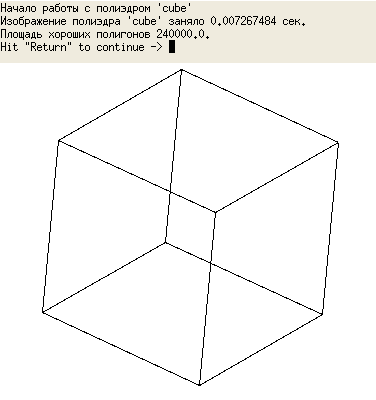
\includegraphics[scale=0.6]{images/222}
\end{center}
\vspace*{-8mm}
\caption{Начало работы с полиэдром куб}\label{fig:term_2}
\end{figure}


